\paragraph{Exercise 1}
Find the minimum state automaton accepting the language denoted by the regular expression: \code{(ab*\|b*a)*}
\begin{figure}[H]
    \centerline{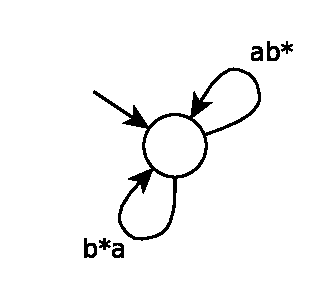
\includegraphics[width=0.3\textwidth]{img/40.pdf}}
\end{figure}
$$
    \Downarrow
$$
\begin{figure}[H]
    \centerline{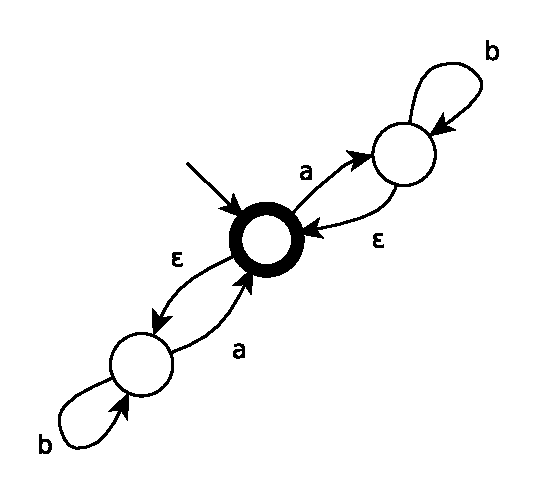
\includegraphics[width=0.5\textwidth]{img/41.pdf}}
\end{figure}
$$
    \Downarrow NFA
$$
\begin{figure}[H]
    \centerline{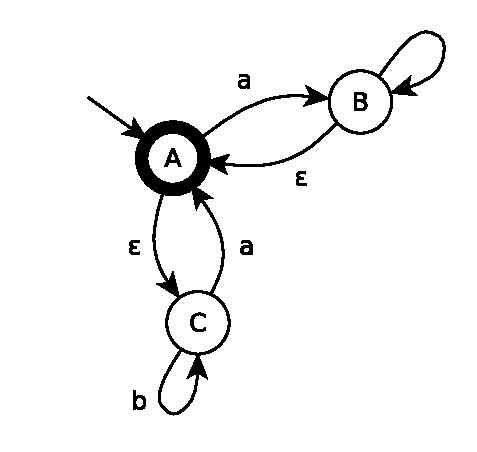
\includegraphics[width=0.4\textwidth]{img/42.pdf}}
\end{figure}
$$
    \Downarrow DFA
$$
\begin{table}[H]
    \centering
    \begin{tabular}{l|l|l}
        & a & b \\ \hline
        A, B & B, A, C & C \\ \hline
        B, A, C & B, A, C & B, A, C \\ \hline
        C & A, C & C \\
    \end{tabular}
\end{table}
$$
    \Downarrow DFA
$$
\begin{figure}[H]
    \centerline{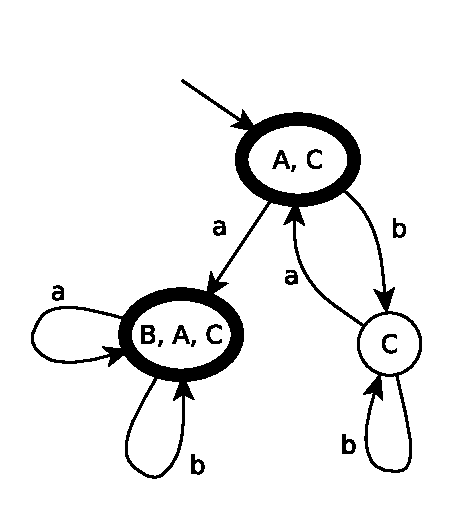
\includegraphics[width=0.3\textwidth]{img/43.pdf}}
\end{figure}
This automaton is already minimum.

\paragraph{Exercise 2}
Verify the equivalence between the following grammars:
\begin{enumerate}
    \item
    $S \to Aa \; | \; Ab \; | \; Sb \; | \; a \; | \; b$ \newline
    $A \to Sa$
    \item
    $S \to aA \; | \; bA \; | \; a \; | \; b$ \newline
    $A \to aS \; | \; bA \; | \; b$
\end{enumerate}

\begin{enumerate}
    \item
    Left regular grammar
    \begin{figure}[H]
        \centerline{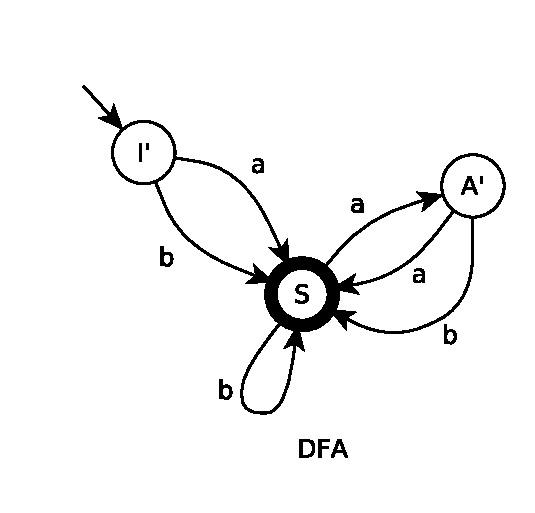
\includegraphics[width=0.4\textwidth]{img/44.pdf}}
    \end{figure}
    $$
        \{I', A', S\}; \{S', B\}
    $$
    \begin{figure}[H]
        \centerline{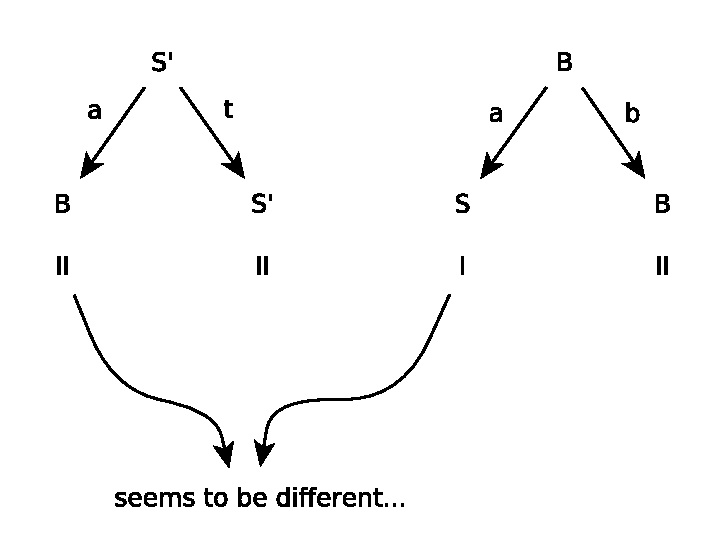
\includegraphics[width=0.3\textwidth]{img/45.pdf}}
    \end{figure}
    \item
    Right regular grammar
    % \begin{figure}[H]
    %     \centerline{\includegraphics[width=0.3\textwidth]{img/46.pdf}}
    % \end{figure}
    \begin{table}[H]
        \centering
        \begin{tabular}{l|l|l}
            & a & b \\ \hline
            S & A, $\Omega$ & A, $\Omega$ \\ \hline
            A, $\Omega$ & S & A, $\Omega$ \\
        \end{tabular}
    \end{table}
    % \begin{figure}[H]
    %     \centerline{\includegraphics[width=0.3\textwidth]{img/47.pdf}}
    % \end{figure}
\end{enumerate}

